\pdfminorversion=4
\documentclass[aspectratio=169]{beamer}

\mode<presentation>
{
  \usetheme{default}
  \usecolortheme{default}
  \usefonttheme{default}
  \setbeamertemplate{navigation symbols}{}
  \setbeamertemplate{caption}[numbered]
  \setbeamertemplate{footline}[frame number]  % or "page number"
  \setbeamercolor{frametitle}{fg=white}
  \setbeamercolor{footline}{fg=black}
}

\usepackage[english]{babel}
\usepackage{inputenc}
\usepackage{tikz}
\usepackage{courier}
\usepackage{array}
\usepackage{bold-extra}
\usepackage{minted}
\usepackage[thicklines]{cancel}
\usepackage{fancyvrb}
\usepackage[normalem]{ulem}

\xdefinecolor{dianablue}{rgb}{0.18,0.24,0.31}
\xdefinecolor{darkblue}{rgb}{0.1,0.1,0.7}
\xdefinecolor{darkgreen}{rgb}{0,0.5,0}
\xdefinecolor{darkgrey}{rgb}{0.35,0.35,0.35}
\xdefinecolor{darkorange}{rgb}{0.8,0.5,0}
\xdefinecolor{darkred}{rgb}{0.7,0,0}
\definecolor{darkgreen}{rgb}{0,0.6,0}
\definecolor{mauve}{rgb}{0.58,0,0.82}

\title[2024-07-24-codas-hep-ml-01]{Machine learning at CoDaS-HEP 2024}
\author{Jim Pivarski}
\institute{Princeton University -- IRIS-HEP}
\date{July 25, 2024}

\usetikzlibrary{shapes.callouts}

\begin{document}

\logo{\pgfputat{\pgfxy(0.11, 7.4)}{\pgfbox[right,base]{\tikz{\filldraw[fill=dianablue, draw=none] (0 cm, 0 cm) rectangle (50 cm, 1 cm);}\mbox{\hspace{-8 cm}
\includegraphics[height=1 cm]{princeton-logo-long.png}\hspace{0.1 cm}\raisebox{0.1 cm}{
\includegraphics[height=0.8 cm]{iris-hep-logo-long.png}}\hspace{0.1 cm}}}}}

\begin{frame}
  \titlepage
\end{frame}

\logo{\pgfputat{\pgfxy(0.11, 7.4)}{\pgfbox[right,base]{\tikz{\filldraw[fill=dianablue, draw=none] (0 cm, 0 cm) rectangle (50 cm, 1 cm);}\mbox{\hspace{-8 cm}
\includegraphics[height=1 cm]{princeton-logo.png}\hspace{0.1 cm}\raisebox{0.1 cm}{
\includegraphics[height=0.8 cm]{iris-hep-logo.png}}\hspace{0.1 cm}}}}}

% Uncomment these lines for an automatically generated outline.
%\begin{frame}{Outline}
%  \tableofcontents
%\end{frame}

% START START START START START START START START START START START START START

\begin{frame}{Now we have two ways to make computer programs}
\vspace{-0.5 cm}

\begin{columns}[t]
\column{0.5\linewidth}
\begin{center}
\Large Craftsmanship

\vspace{0.25 cm}
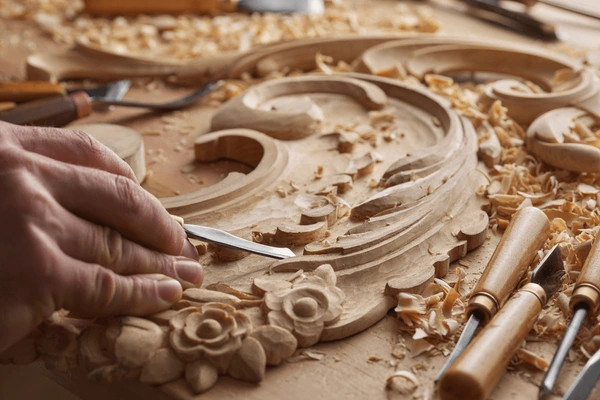
\includegraphics[width=0.8\linewidth]{img/craftsmanship.jpg}

\normalsize
\vspace{0.25 cm}
\begin{itemize}
\item Programming ``by hand''
\item Allows for precise control
\item Complexity limited by a human mind or a team's ability to communicate
\end{itemize}
\end{center}

\column{0.5\linewidth}
\begin{center}
\Large Farming

\vspace{0.25 cm}
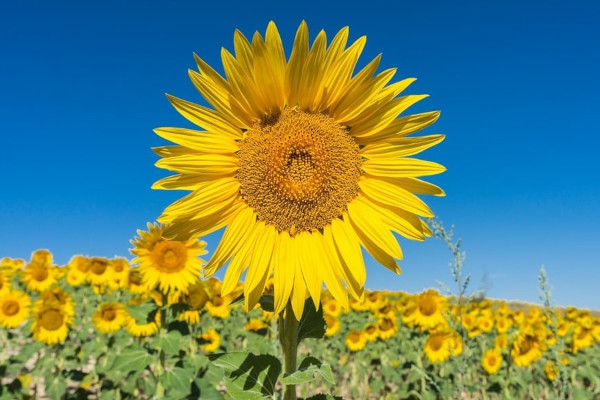
\includegraphics[width=0.8\linewidth]{img/farming.jpg}

\normalsize
\vspace{0.25 cm}
\begin{itemize}
\item Machine learning
\item Allows for extremely nuanced solutions
\item Still needs human help to steer it toward the ``right'' solution
\end{itemize}
\end{center}

\end{columns}
\end{frame}

\begin{frame}{Machine learning in a nutshell}
\vspace{0.4 cm}
\Large

Write an algorithm that generates output that depends on a huge number of internal parameters.

\vspace{0.5 cm}
\uncover<2->{Vary those parameters until the algorithm returns the expected result (supervised learning) or until it finds patterns according to some desired metric (unsupervised learning).}

\vspace{0.5 cm}
\uncover<3->{Then use the trained algorithm on new problems.}

\vspace{0.5 cm}
\uncover<4->{\textcolor{darkblue}{If this sounds like a simple curve fit to data, you're right.}}
\end{frame}

\begin{frame}{Goals of this mini-course}
\vspace{0.4 cm}
\Large

\begin{enumerate}\setlength{\itemsep}{0.5 cm}
\item Understand how your physics background prepares you for machine learning.
\item Don't approach it as a black box/dark art.
\item Get a little familiar with some common tools and techniques.
\end{enumerate}
\end{frame}

\begin{frame}{A very brief history of HEP and ML}
\Large
\vspace{0.5 cm}
\begin{columns}
\column{0.5\linewidth}
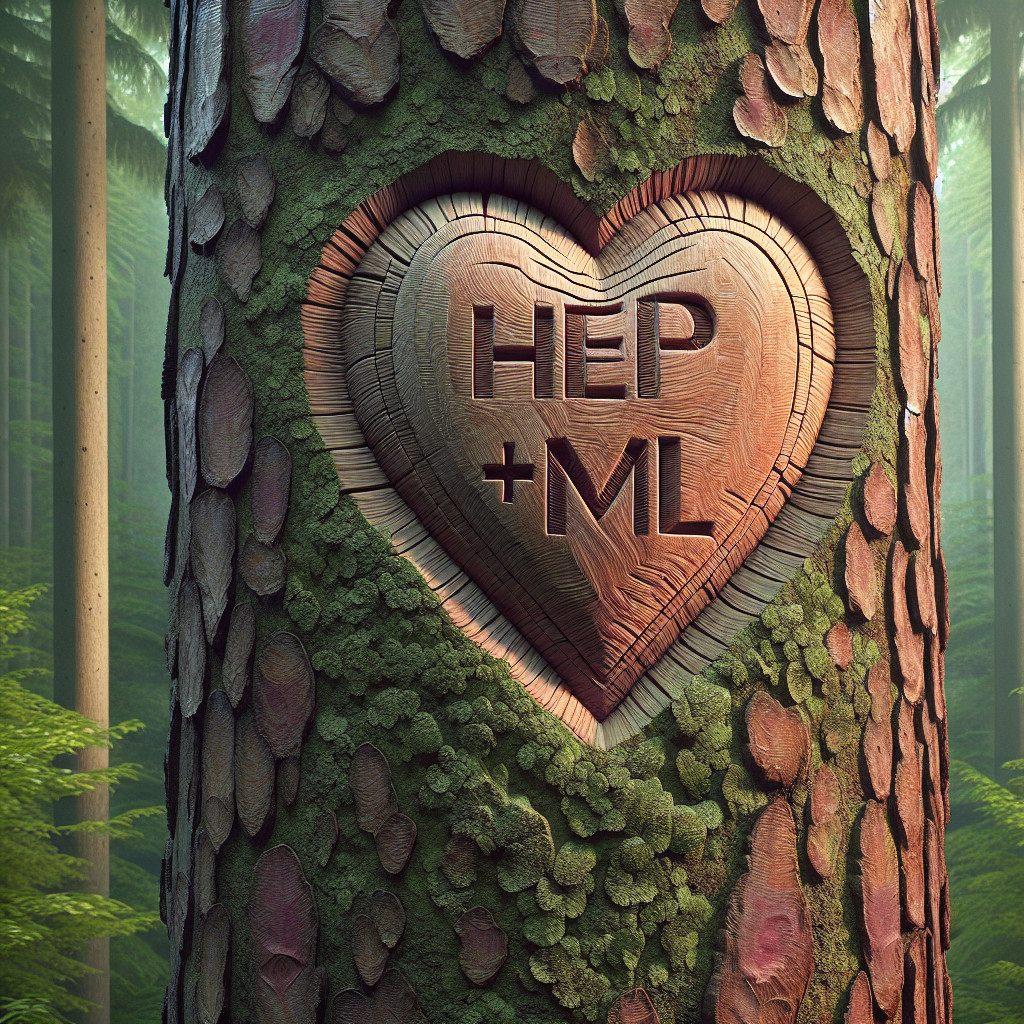
\includegraphics[width=\linewidth]{img/hep-plus-ml.jpg}

\column{0.5\linewidth}
Main point: High Energy Physics (HEP) has always needed Machine Learning (ML).

\vspace{0.5 cm}
It's just becoming {\it possible} now.
\end{columns}
\end{frame}

\begin{frame}{First HEP experiments adopted computers in a major way}
\vspace{0.35 cm}
\large

Late 1940's---early 1950's was the ``beginning'' of HEP as we know it:

\vspace{0.25 cm}
\begin{itemize}
\item Accelerators provided higher energy with higher flux than observed in nature.
\item Collisions with fixed targets produced new particles to discover.
\item Computers quantified particle trajectories, reconstructed invisible (neutral) particles, and rejected backgrounds.
\end{itemize}

\normalsize
\vspace{0.35 cm}
Example: Luis Alvarez's group \textcolor{darkgreen}{\$9M} accelerator, \textcolor{darkgreen}{\$2M} bubble chamber, \textcolor{darkgreen}{\$0.2M} IBM 650.

\vspace{0.25 cm}
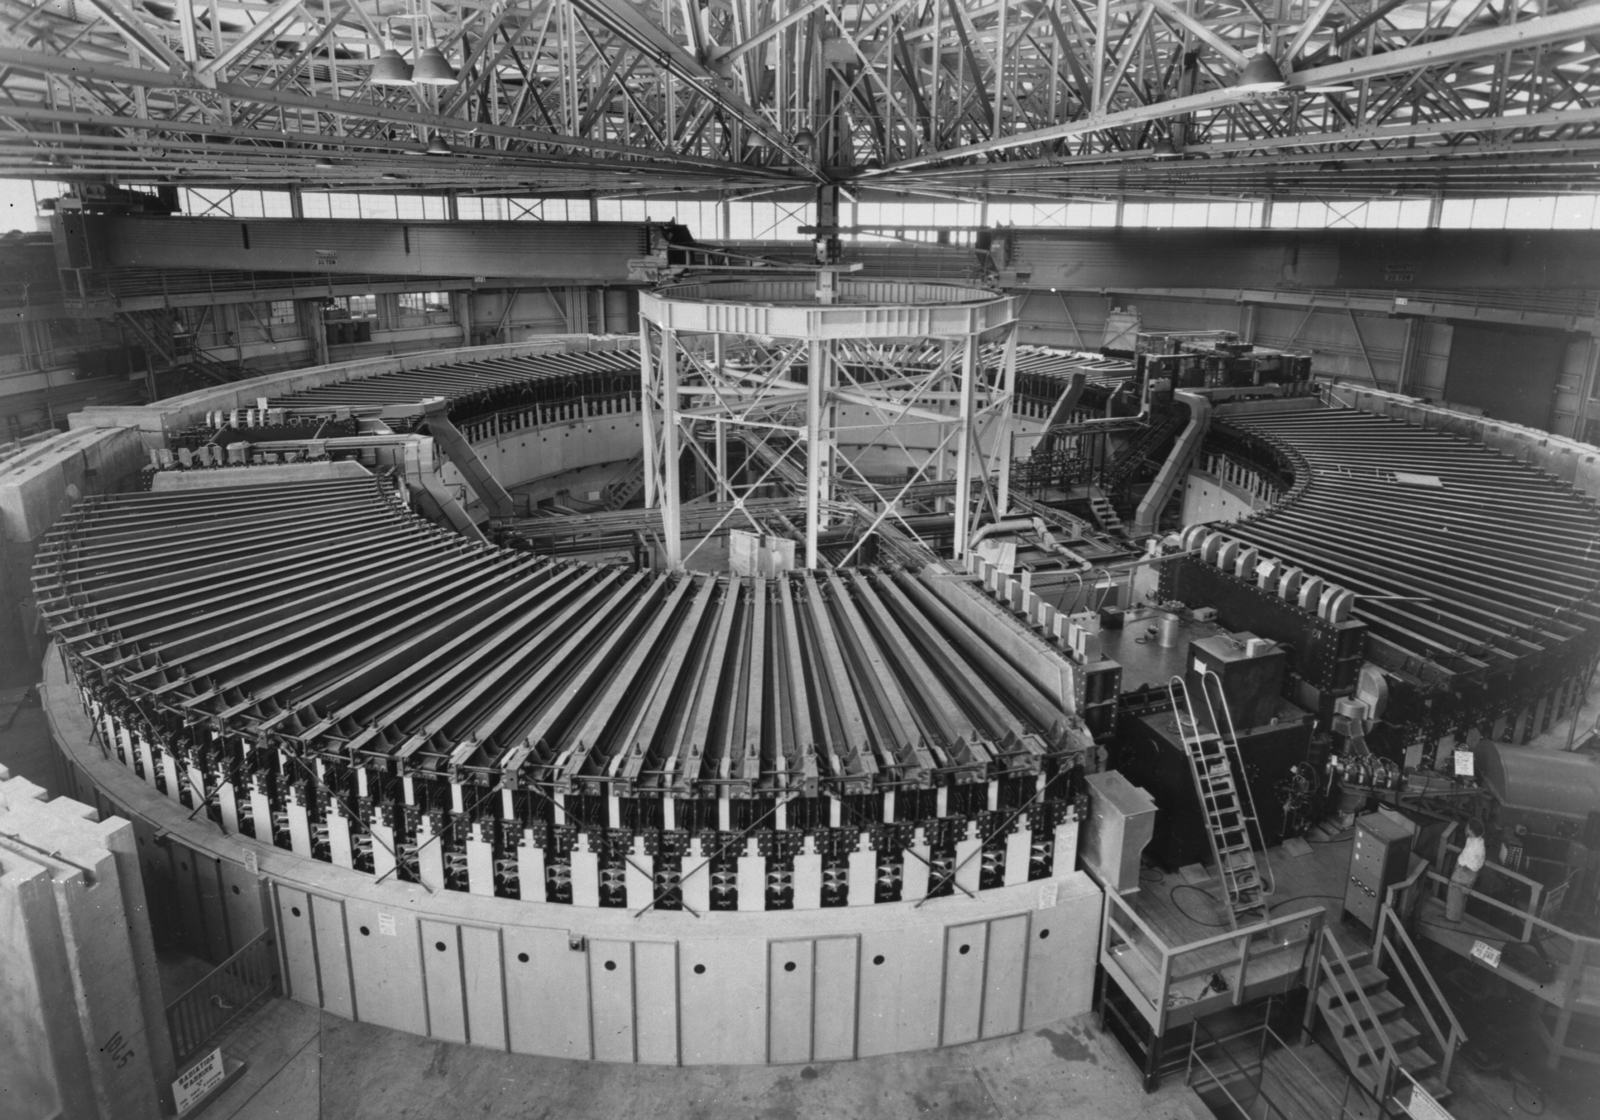
\includegraphics[height=3 cm]{img/overall-view-of-bevatron-magnet-photograph-taken-september-6-1955-bevatron-088cb0-1600.jpg}
\hfill 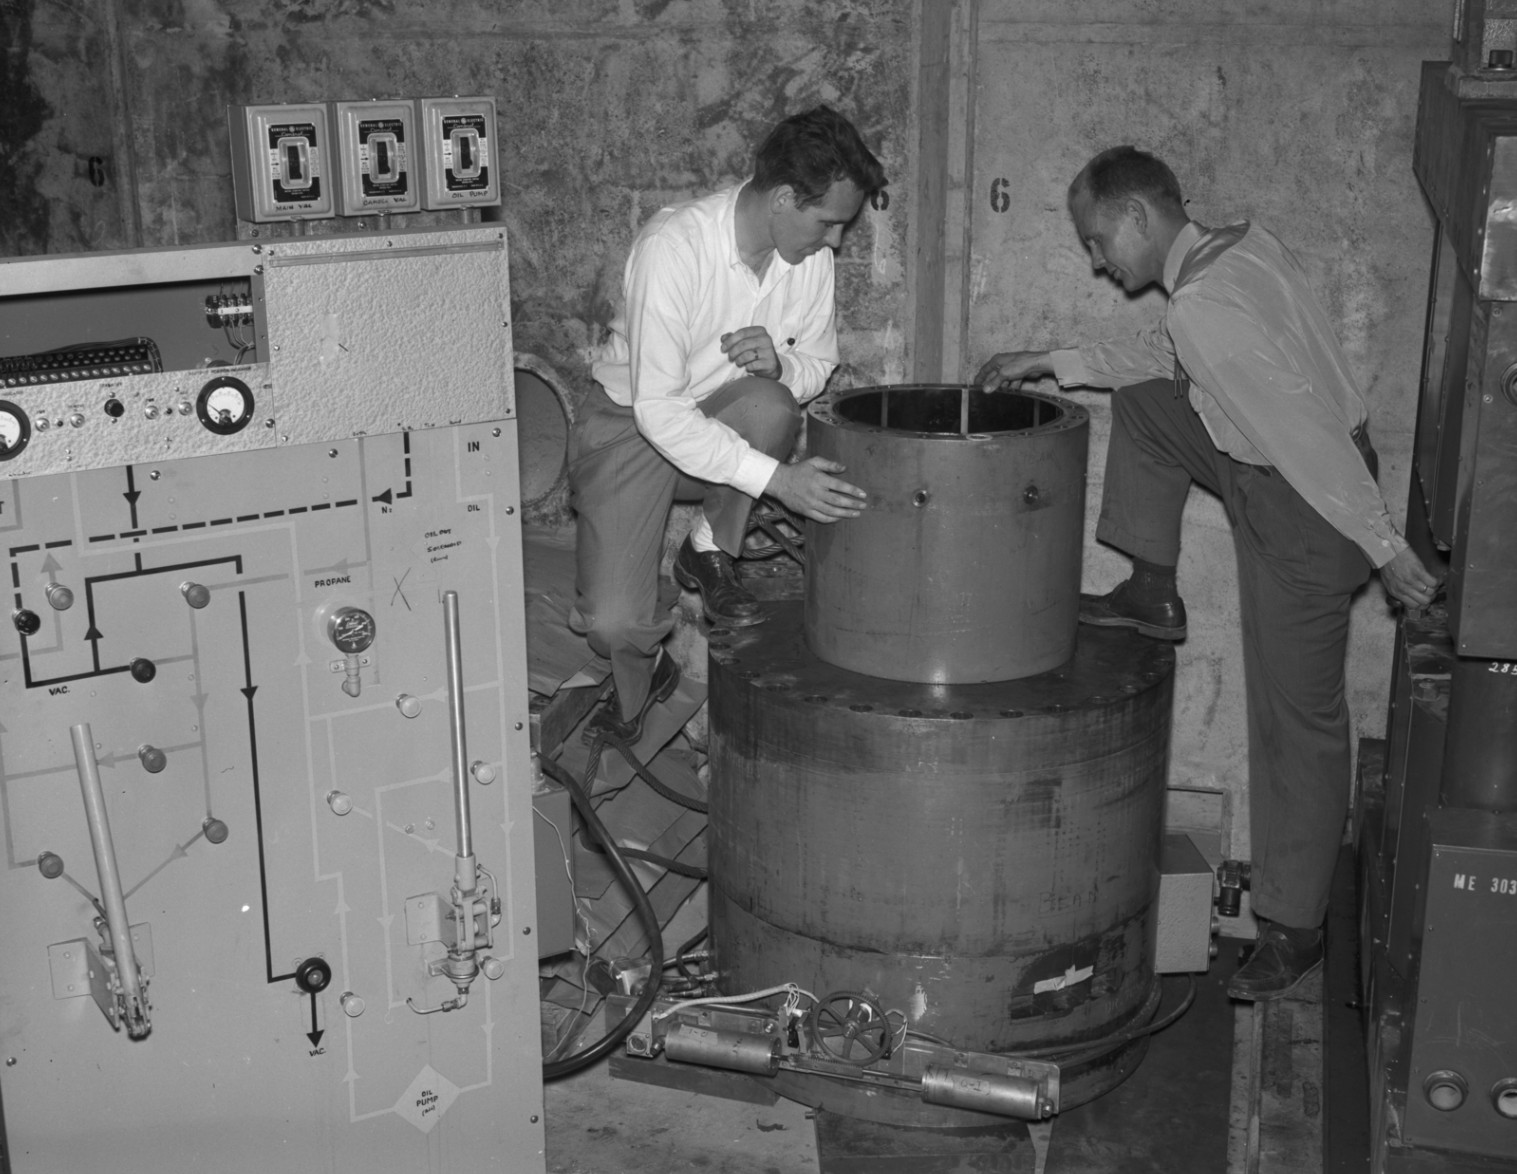
\includegraphics[height=3 cm]{img/alvarez-group-bubble-chamber.jpg}
\hfill 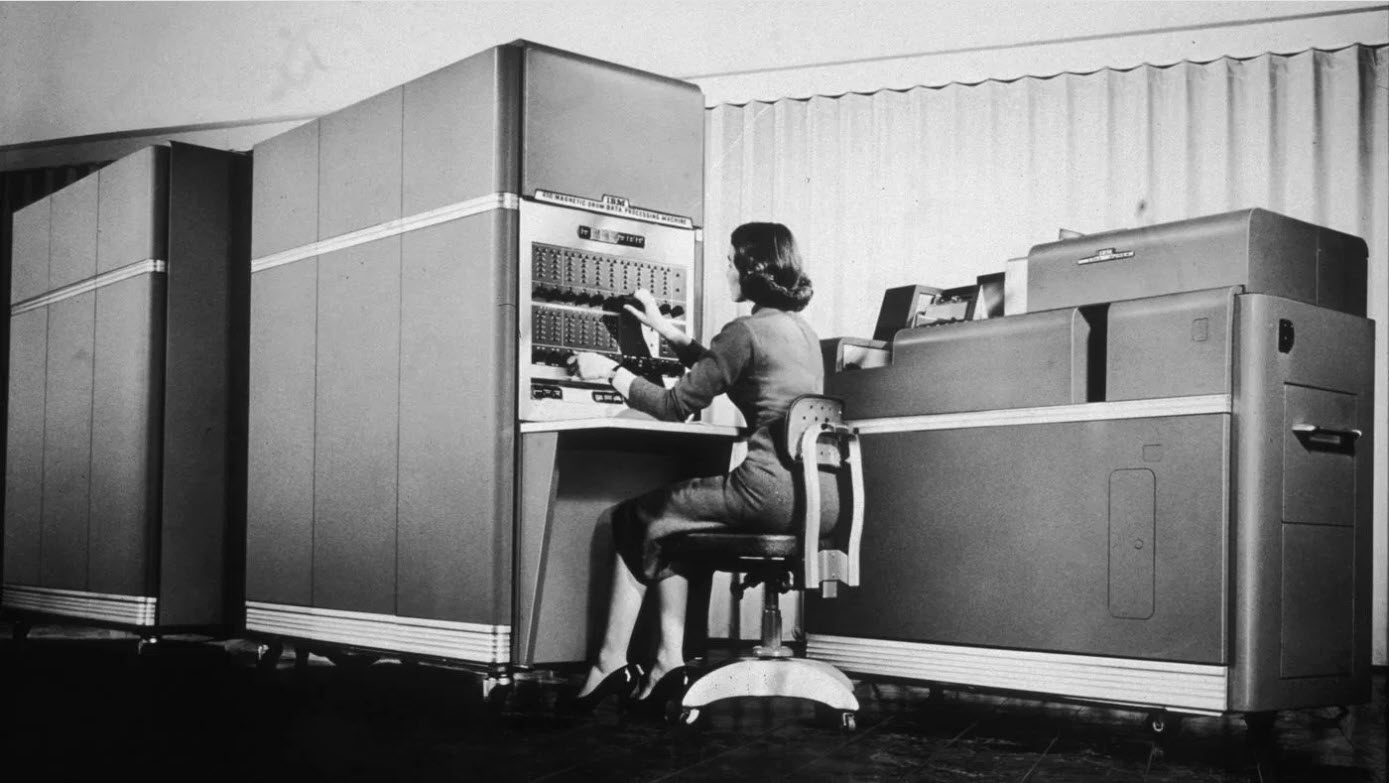
\includegraphics[height=3 cm]{img/ibm-650.jpg}
\end{frame}

\begin{frame}{Identifying tracks was beyond the capabilities of software}
\vspace{0.35 cm}
\begin{columns}
\column{0.7\linewidth}
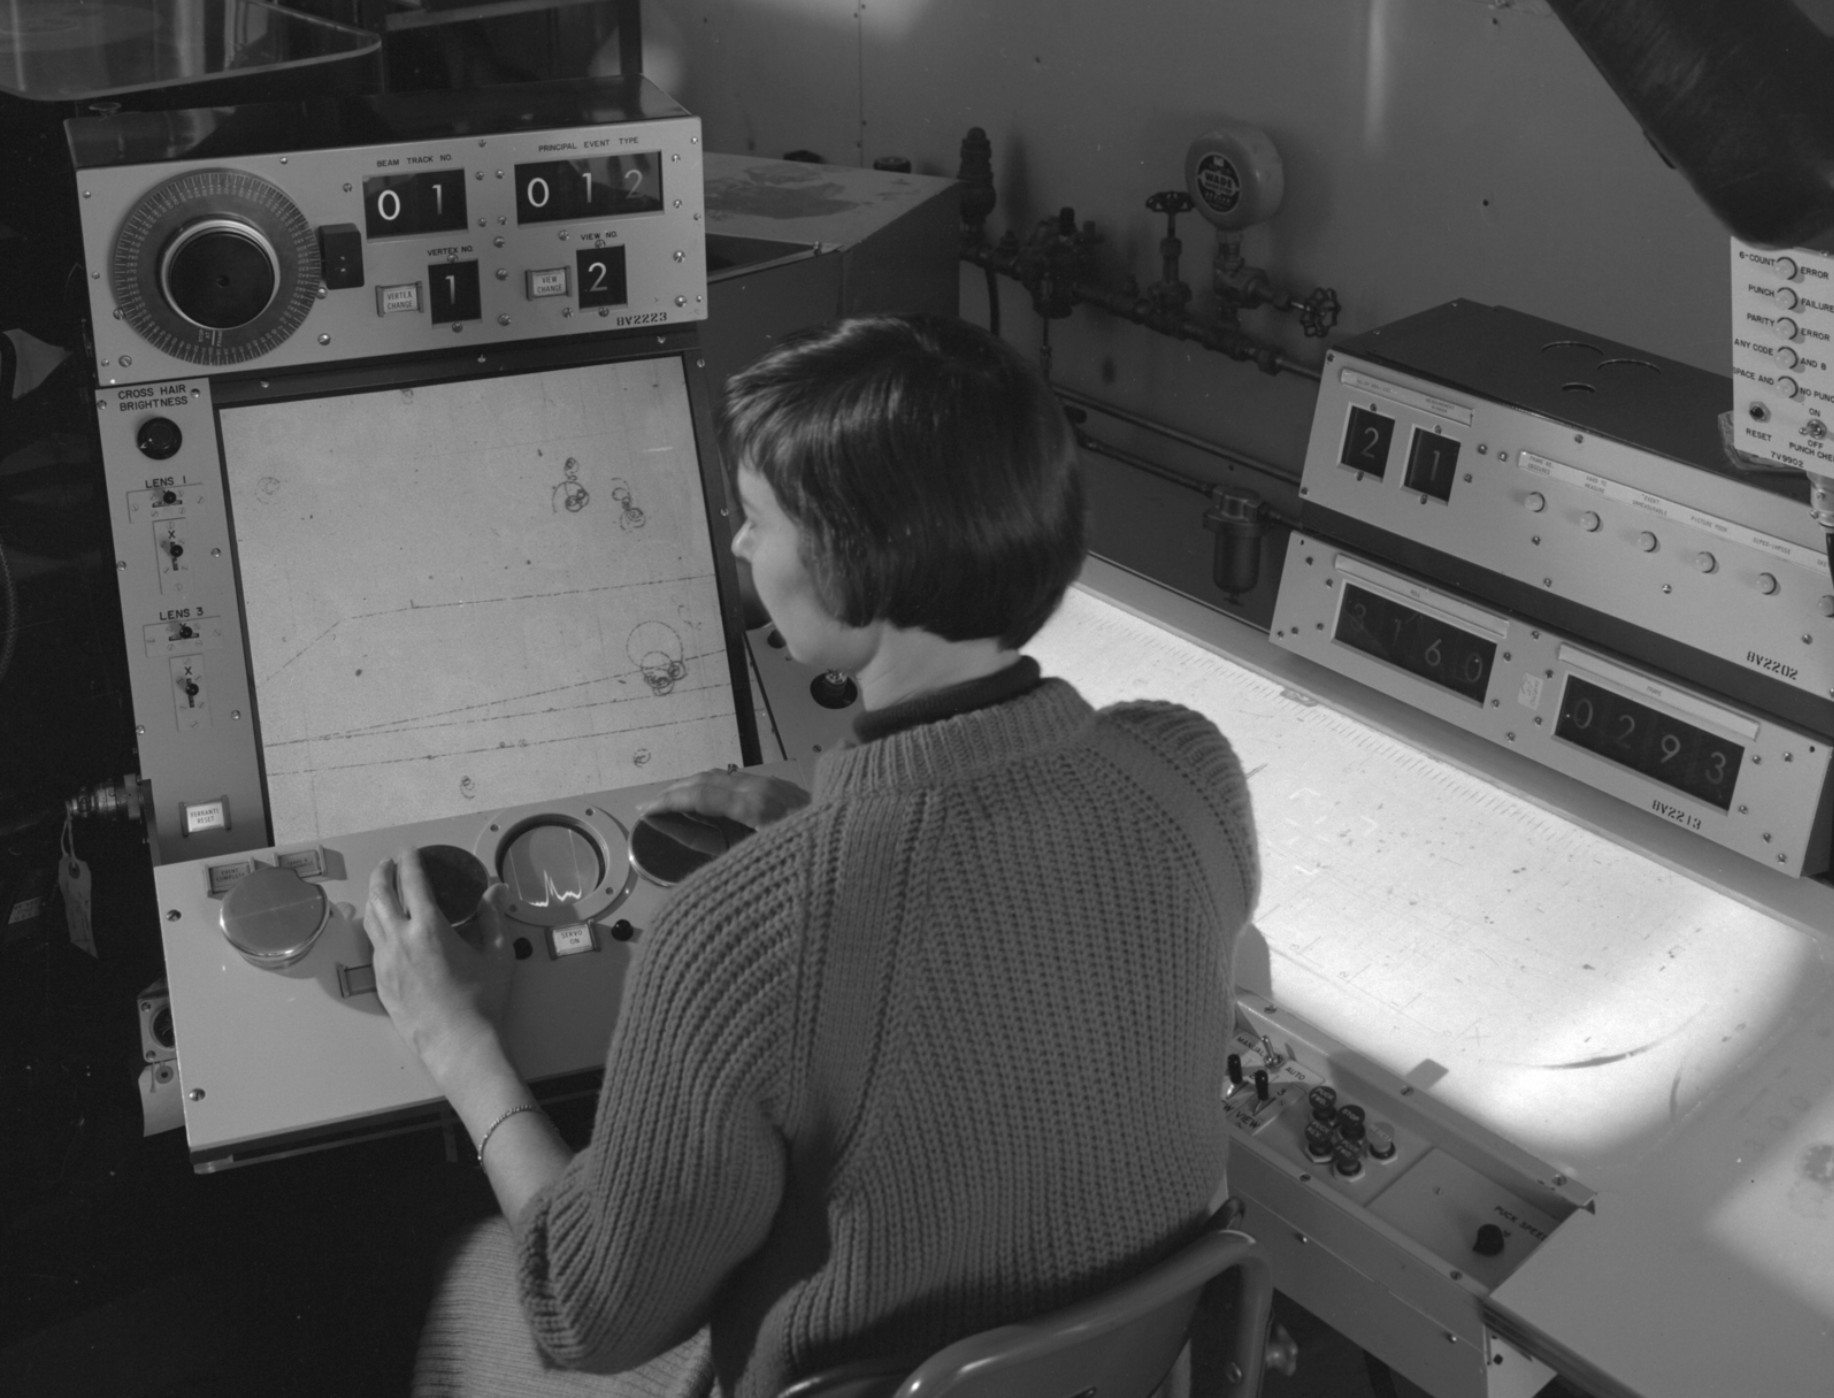
\includegraphics[width=\linewidth]{img/franckenstein-3.jpg}

\column{0.3\linewidth}
\vspace{-0.5 cm}
\begin{center}
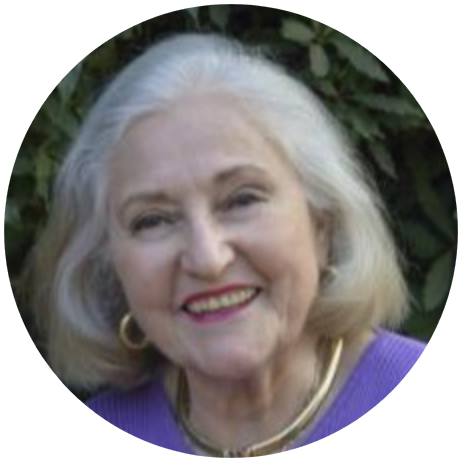
\includegraphics[width=0.5\linewidth]{img/madeleine-isenberg-SCANNER.png}

\scriptsize
Madeleine (n\'ee Goldstein) Isenberg, UCLA class of '65
\end{center}

\begin{minipage}{\linewidth}
\scriptsize
``We scanners would review each frame of film, and per the brief instructions we had been given, looked for any `unusual activity.'

\vspace{0.25 cm}
``The scanner had to use both hands, a joystick in each, and turn them clockwise or anti-clockwise, to align a double crosshair cursor at several sequential positions on a track.''

\vspace{0.25 cm}
\tiny
\textcolor{blue}{\url{https://www.physics.ucla.edu/marty/HighEnergyPhysics.pdf}}
\end{minipage}
\end{columns}
\end{frame}

\begin{frame}{Fast pattern recognition tasks are an essential part of HEP}
\vspace{0.4 cm}
\begin{columns}
\column{0.25\linewidth}
\only<1>{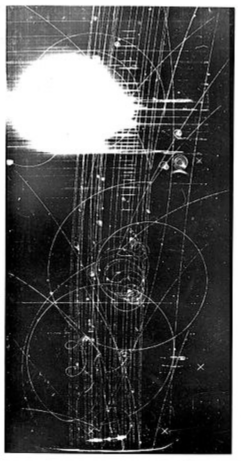
\includegraphics[height=7.5 cm]{img/bubble-chamber-photo-0.pdf}}\only<2->{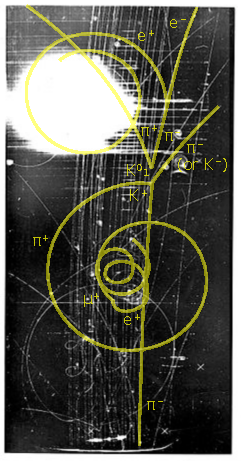
\includegraphics[height=7.5 cm]{img/bubble-chamber-photo.pdf}}

\column{0.2\linewidth}
Detectors make unlabeled event displays.

\vspace{0.5 cm}
\uncover<2->{Once labeled, events can be processed in bulk.}

\vspace{0.5 cm}
\uncover<3->{Capacity for discovery scales with the number of labeled events.}

\column{0.4\linewidth}
\uncover<3->{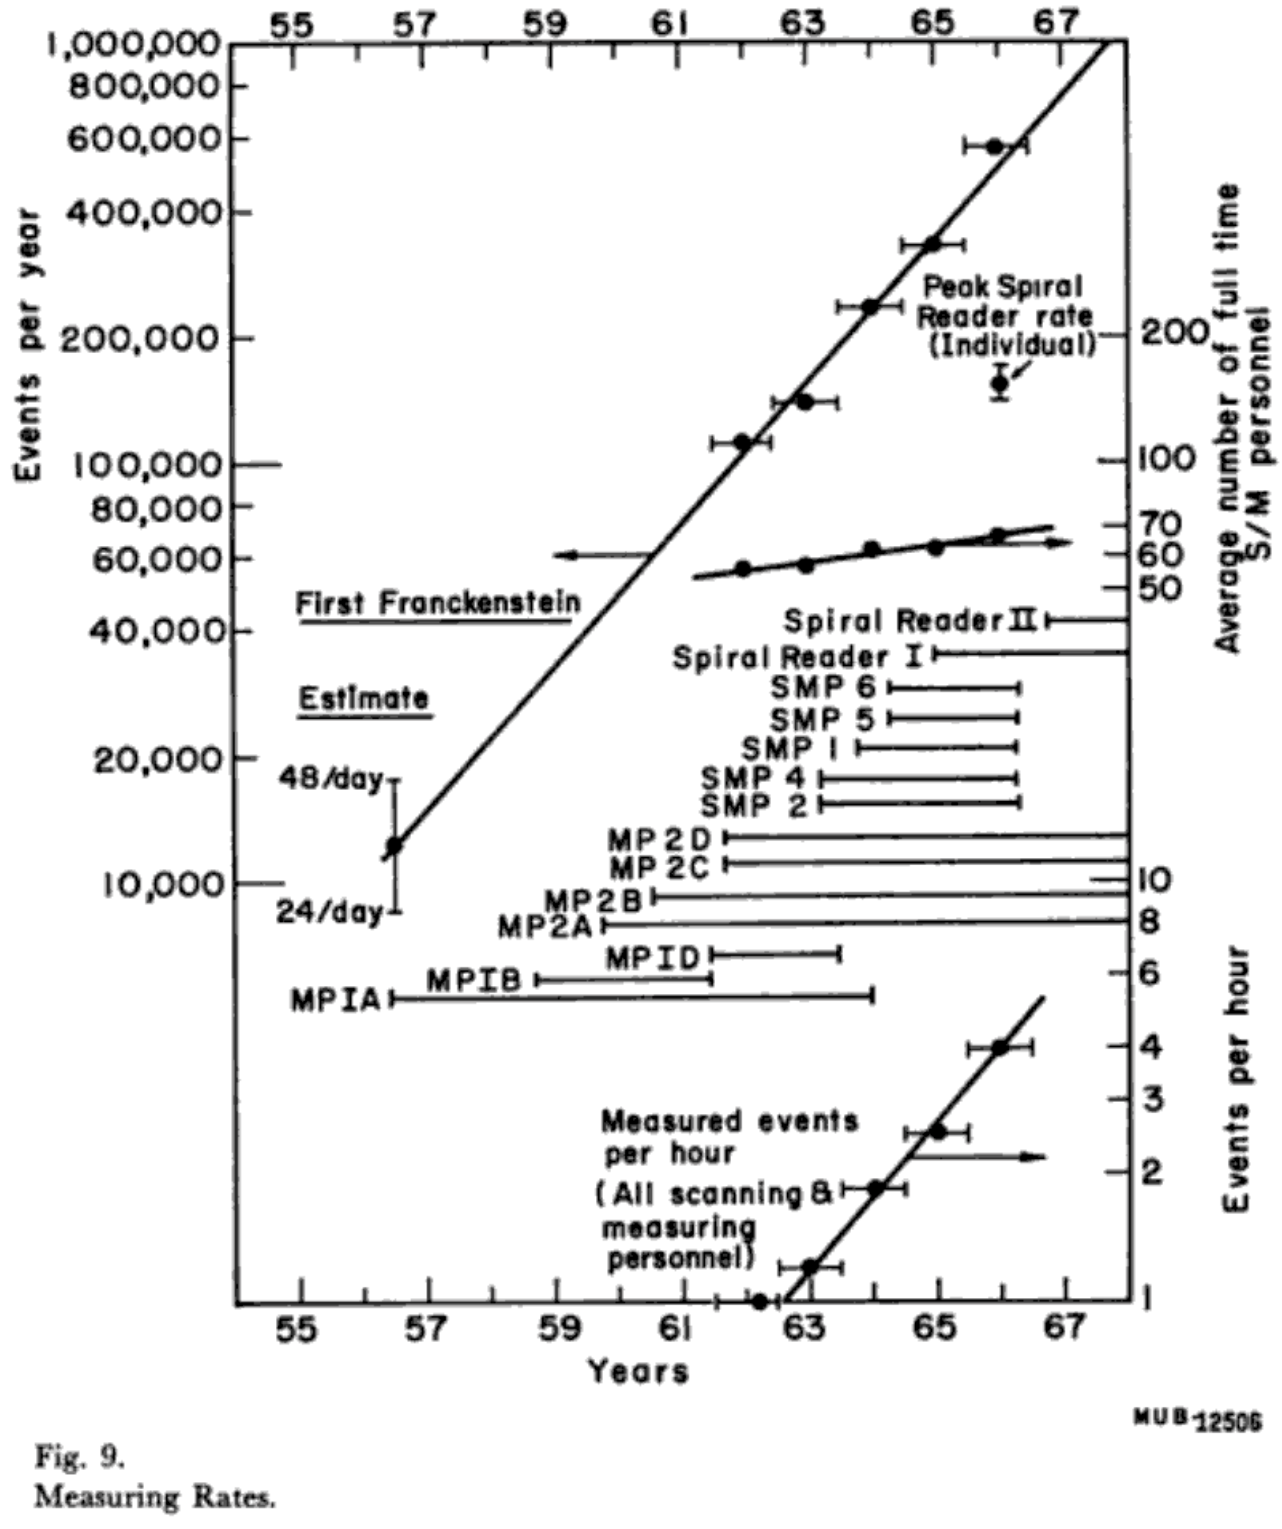
\includegraphics[height=7.5 cm]{img/scaleup.png}}
\end{columns}
\end{frame}

\begin{frame}{Pattern recognition had to be automated to reach today's rates}
\vspace{0.25 cm}
\begin{columns}
\column{1.1\linewidth}
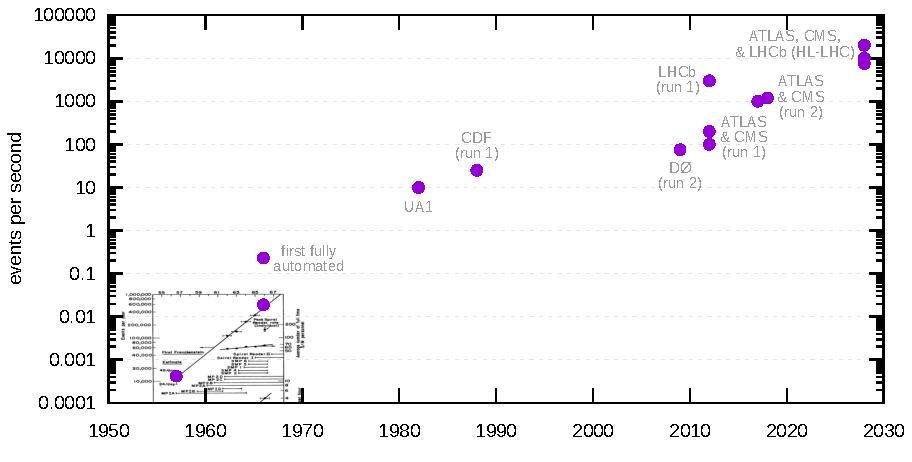
\includegraphics[width=\linewidth]{img/event-rates.pdf}
\end{columns}
\end{frame}

\begin{frame}{\mbox{ }}
\vspace{0.5 cm}
\Large

Until recently, most HEP pattern-recognition consisted of hand-written heuristics (some still is).

\vspace{1 cm}
\uncover<2->{The history of Artificial Intelligence (AI) is also split between what we would now call hand-written algorithms and learned algorithms.}
\end{frame}

\begin{frame}{Symbolic AI versus Connectionist AI}
\vspace{-0.7 cm}

\begin{columns}[t]
\column{0.5\linewidth}
\begin{center}
\Large Symbolic

\vspace{0.25 cm}
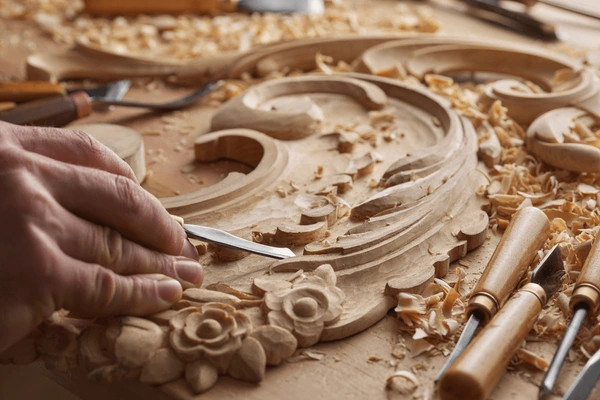
\includegraphics[width=0.8\linewidth]{img/craftsmanship.jpg}

\normalsize
\vspace{0.25 cm}
\begin{itemize}
\item Symbol manipulation and logic
\item Searches through problem-space
\item Hand-written common-sense rules
\end{itemize}

Examples: parsing, theorem-proving, chess-playing, expert systems
\end{center}

\column{0.5\linewidth}
\begin{center}
\Large Connectionist

\vspace{0.25 cm}
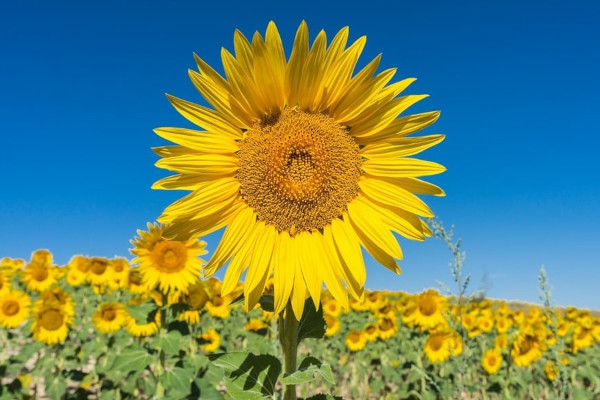
\includegraphics[width=0.8\linewidth]{img/farming.jpg}

\normalsize
\vspace{0.25 cm}
\begin{itemize}
\item Stimulus correlated to response only by strengths of internal connections
\item No \underline{\it explicit} symbols or rules
\item \underline{\it Effective} symbols/rules may arise
\end{itemize}

Examples: neural networks
\end{center}

\end{columns}
\end{frame}

\begin{frame}{Connectionism started early}
\small
\vspace{0.2 cm}
\begin{columns}
\column{0.4\linewidth}
\includegraphics[width=\linewidth]{img/330-PSA-80-60_\(USN_710739\)_\(20897323365\).jpg}

\vspace{0.2 cm}
Theory: Pitts \& McCullock (1943).

\vspace{0.2 cm}
Rosenblatt's perceptron machine (1958) attempted to recognize images of letters by adjusting free parameters with motors.

\vspace{0.2 cm}
\mbox{\textcolor{darkorange}{\bf Made extravagant claims; reality hit hard.}\hspace{-1 cm}}

\column{0.6\linewidth}
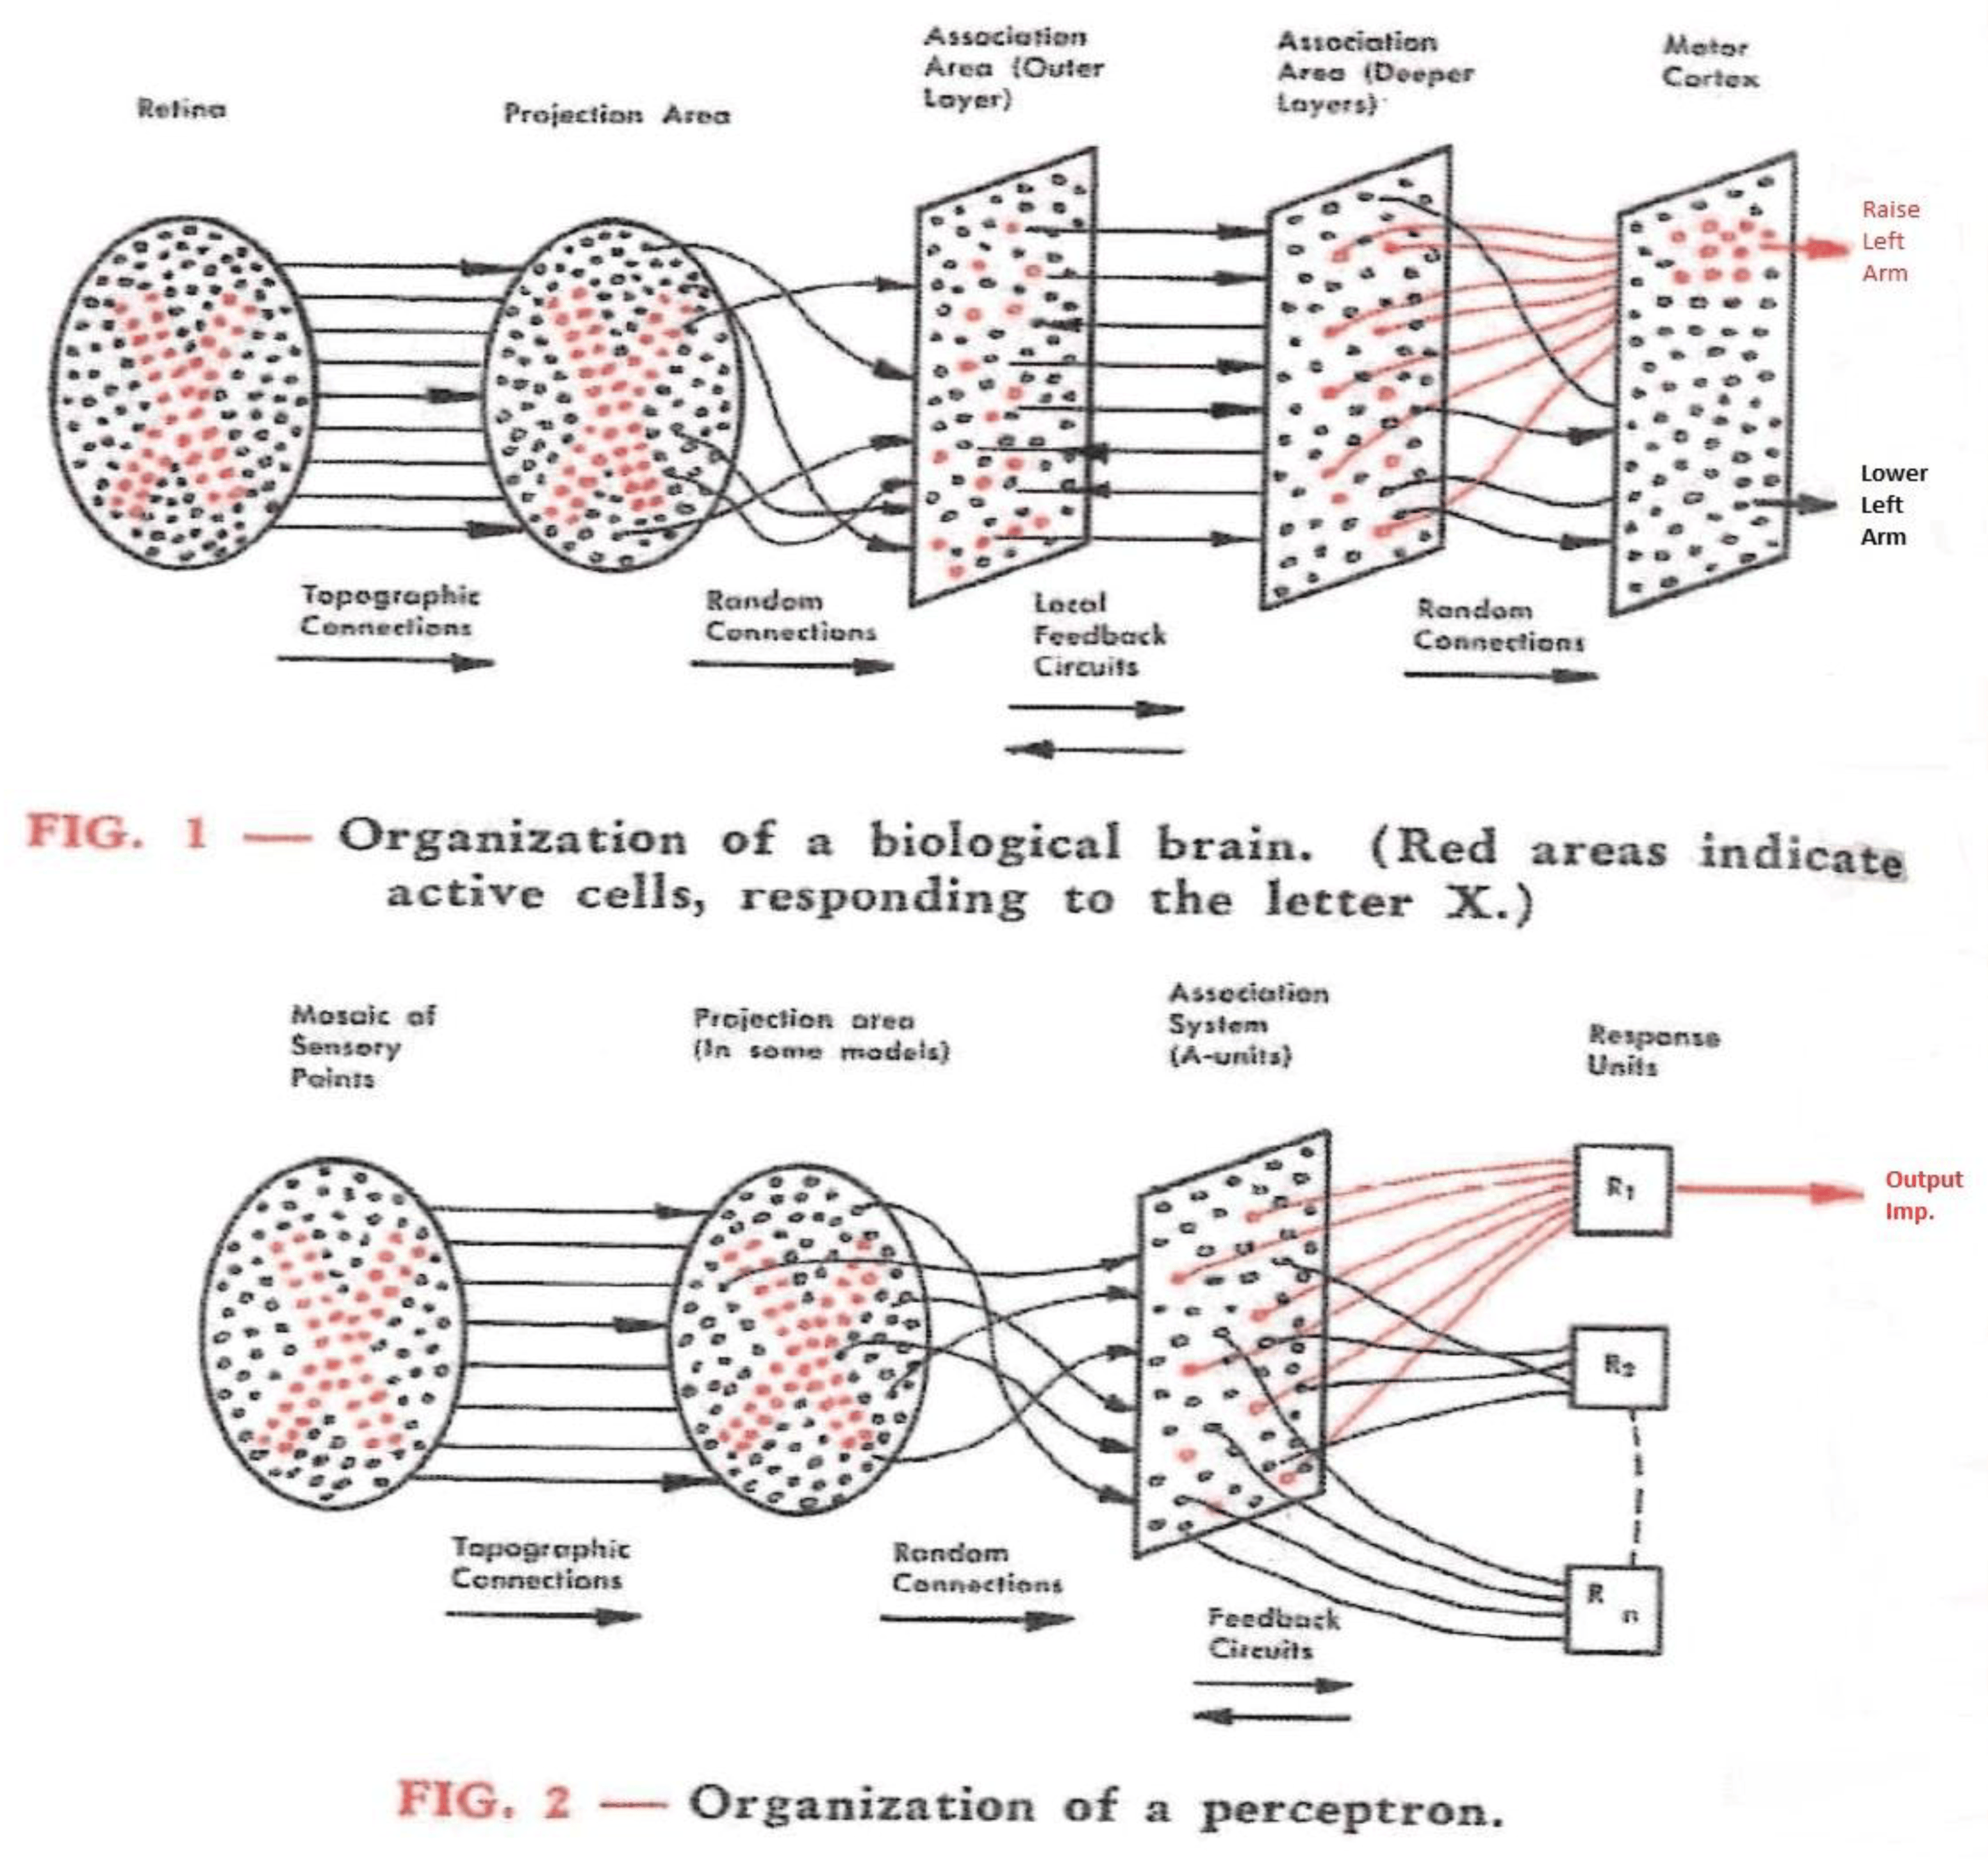
\includegraphics[width=\linewidth]{img/Organization_of_a_biological_brain_and_a_perceptron.png}
\end{columns}
\end{frame}

\begin{frame}{The ups and downs of AI: \only<1>{as mentioned in books}\only<2>{according to Henry Kautz (funding)}}
\vspace{0.2 cm}
\begin{columns}
\column{1.1\linewidth}
\only<1>{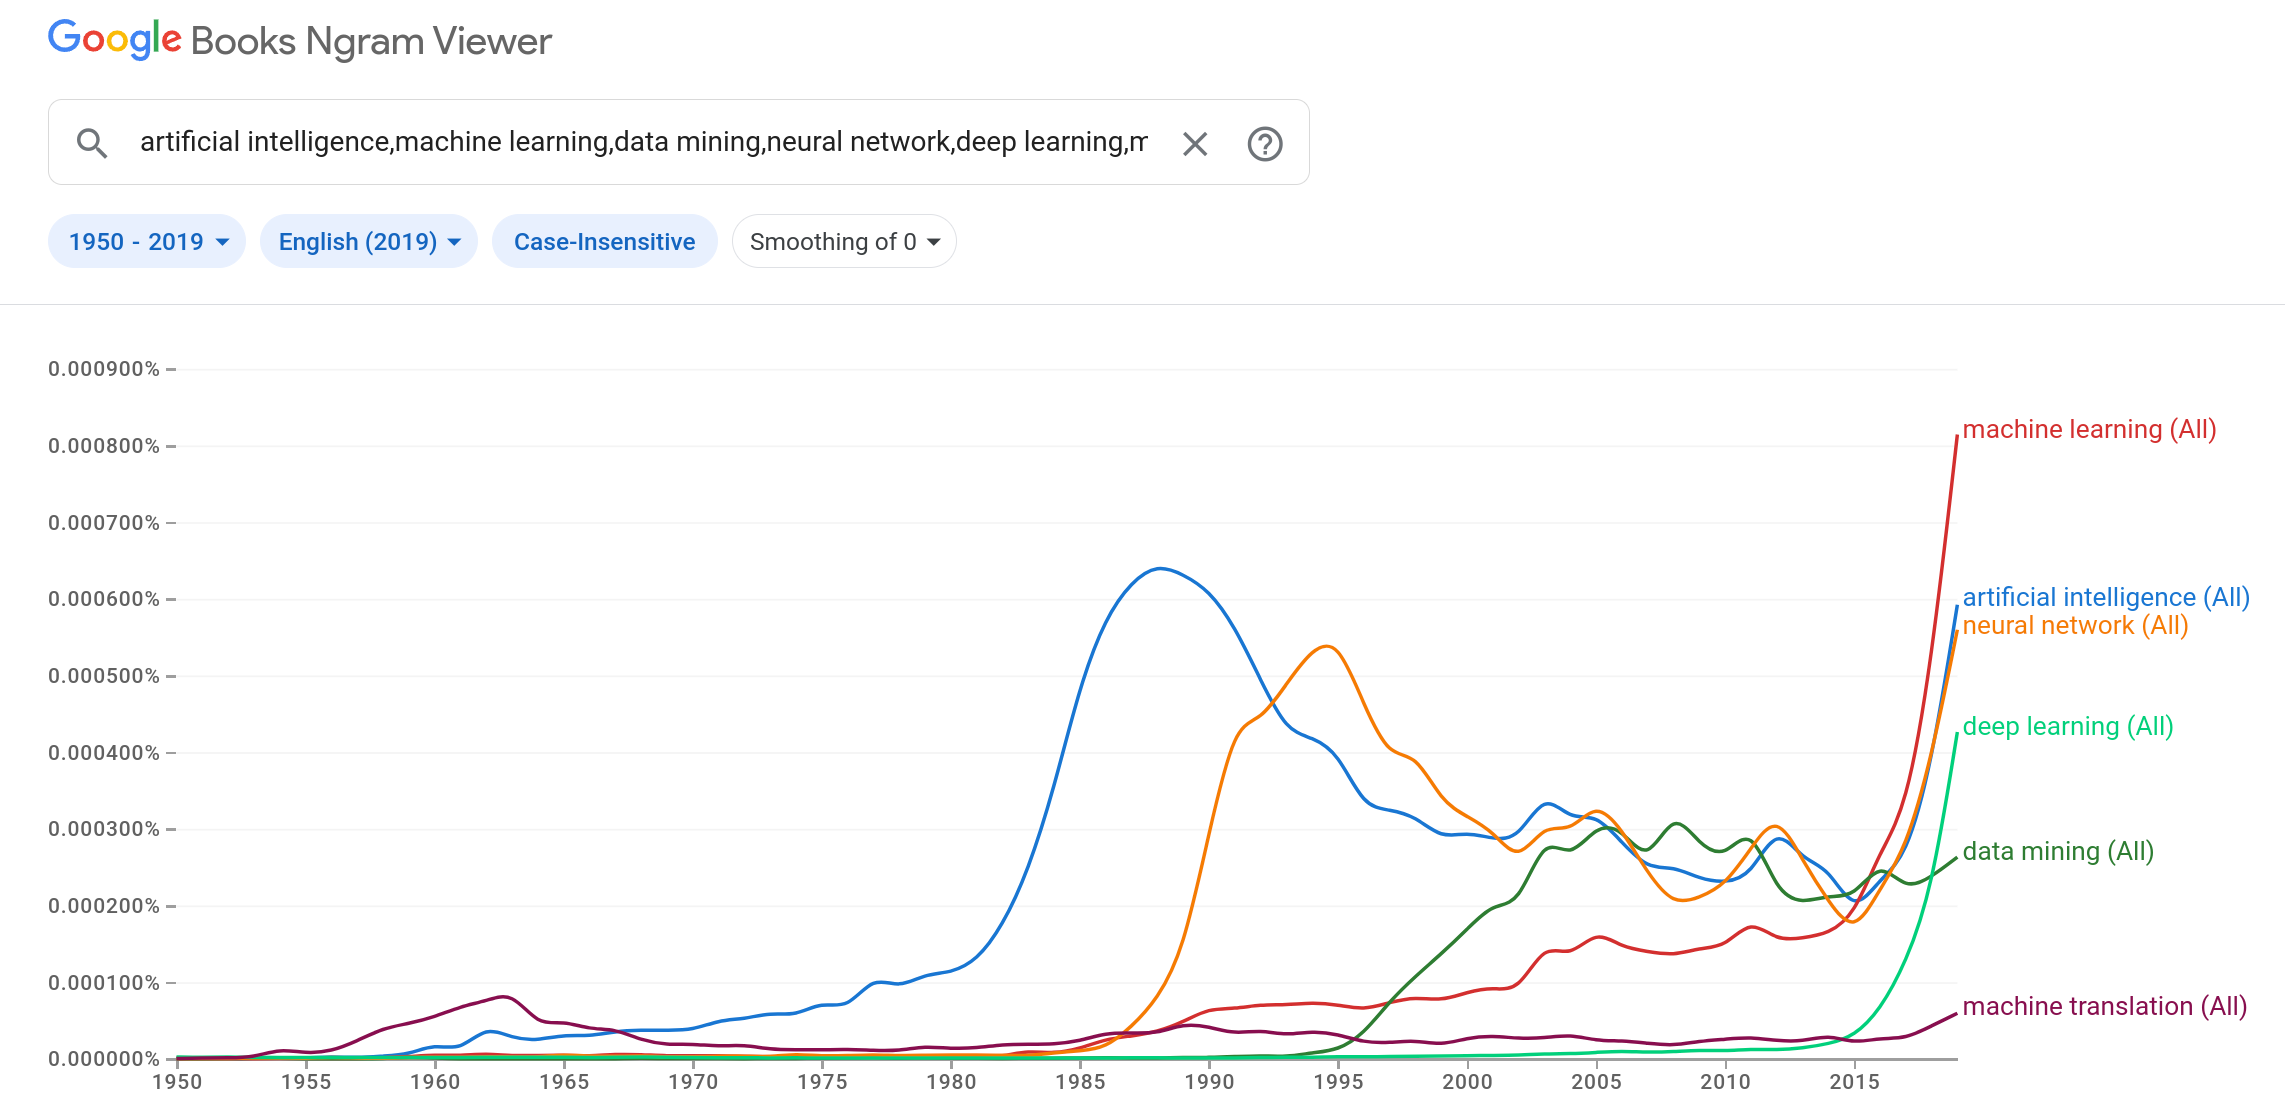
\includegraphics[width=\linewidth]{img/ups-and-downs-of-ai.png}}\only<2>{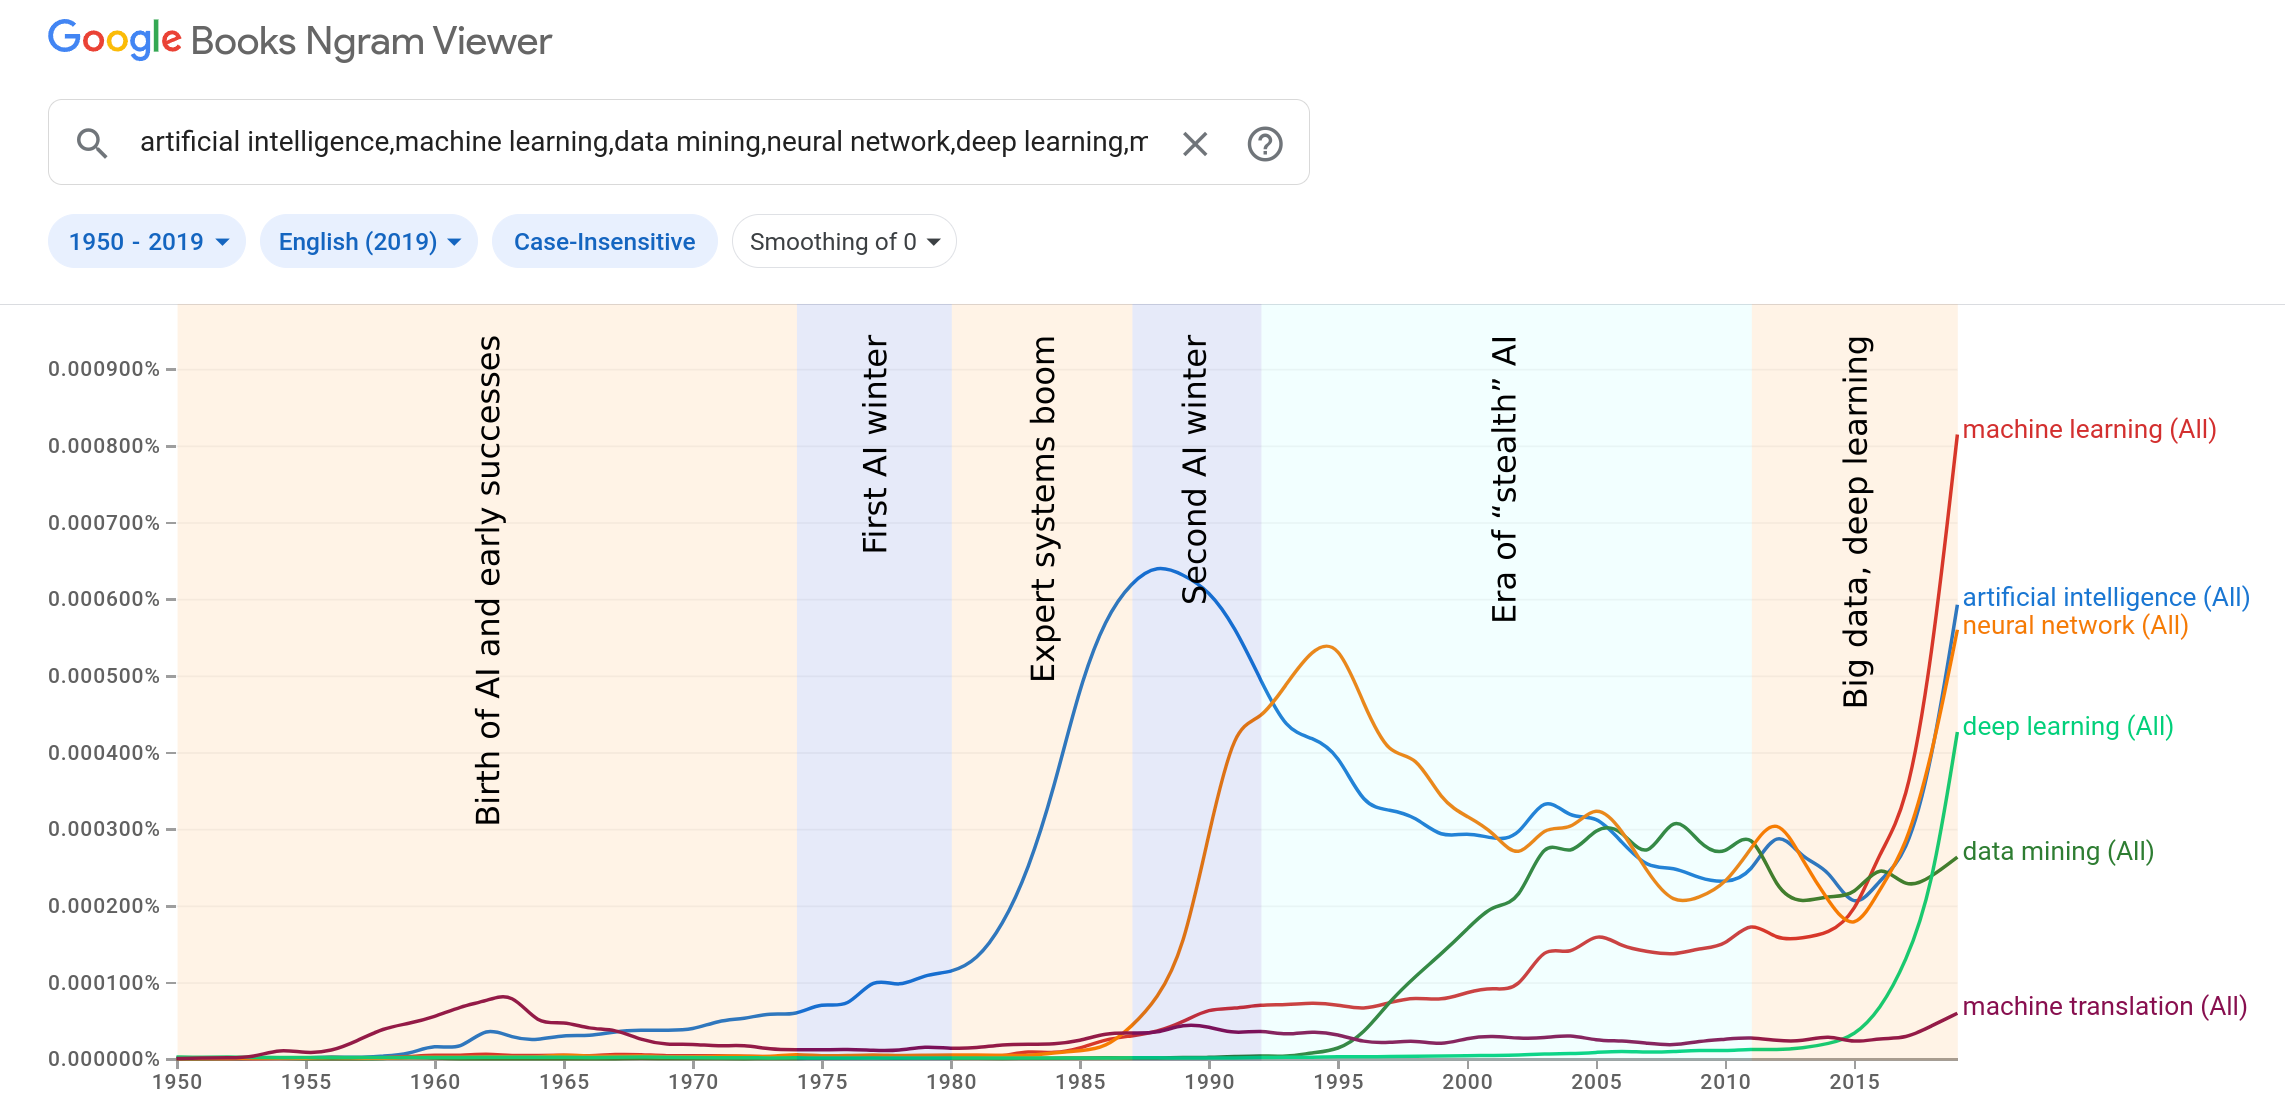
\includegraphics[width=\linewidth]{img/ups-and-downs-of-ai-overlay.png}}
\end{columns}
\end{frame}

\begin{frame}{The ups and downs of AI: in conference attendance}
\vspace{0.5 cm}
\begin{columns}
\column{1.1\linewidth}
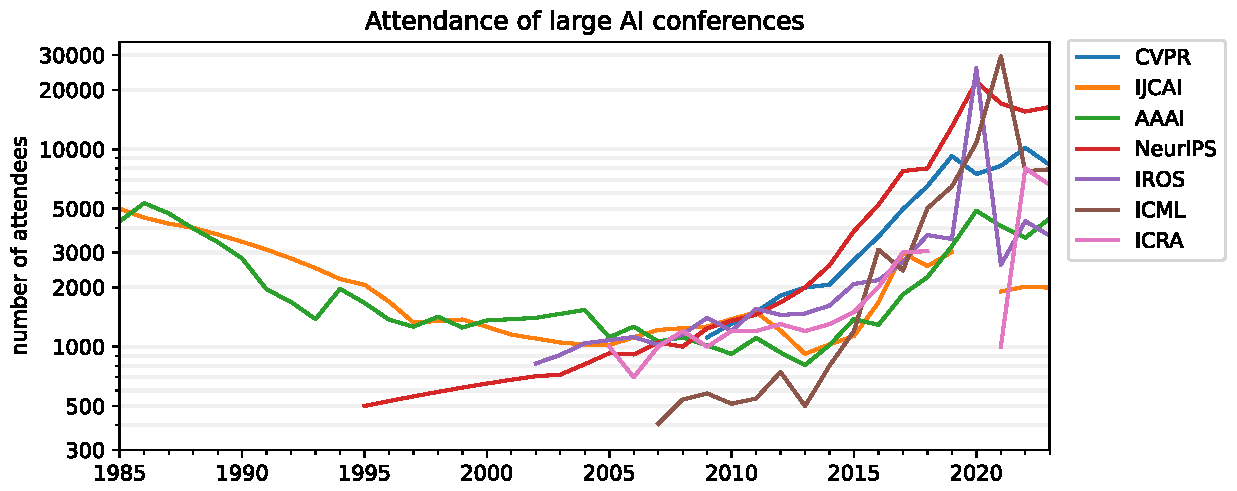
\includegraphics[width=\linewidth]{img/AI-conference-attendance.pdf}
\end{columns}
\end{frame}

\begin{frame}{The ups and downs of AI: among physicists at CHEP}
\vspace{0.25 cm}
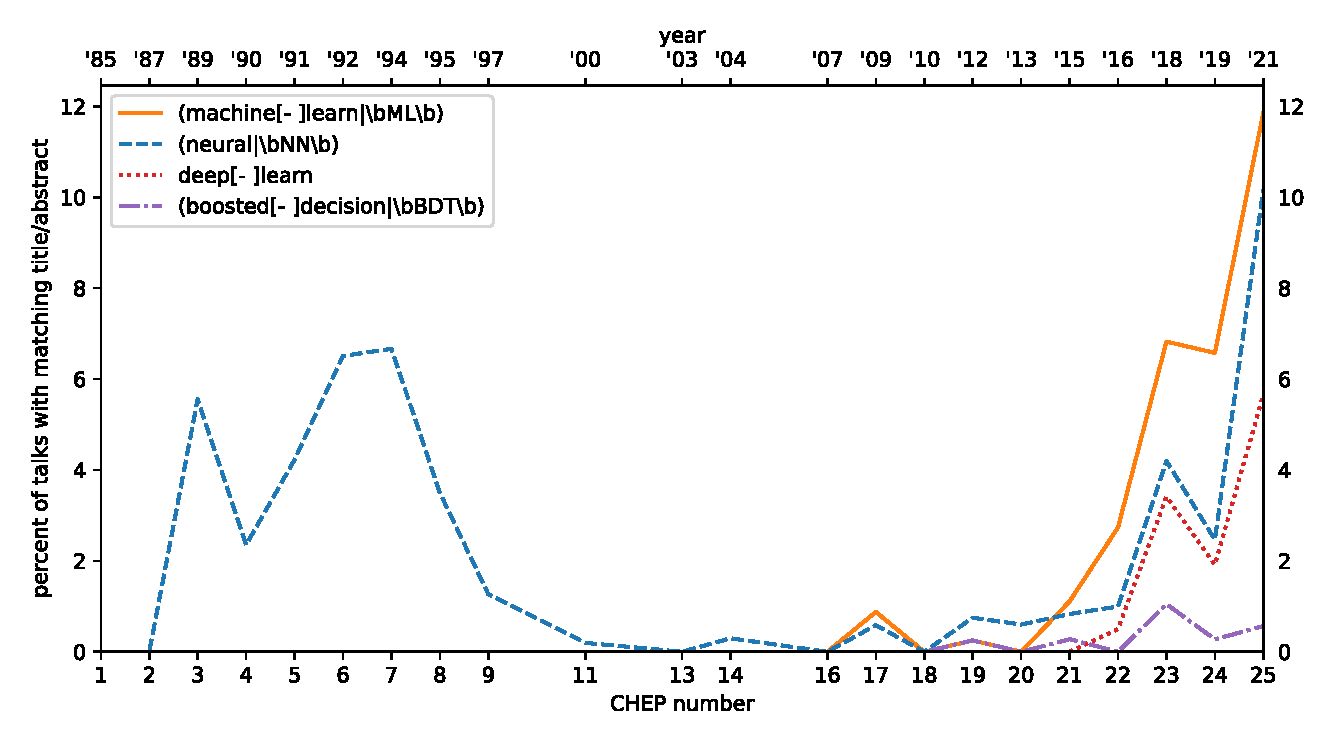
\includegraphics[width=\linewidth]{img/chep-papers-ml.pdf}
\end{frame}



\end{document}
